%! TeX root = ../Parte1.tex

\section{Phishing}

\begin{myframe}{Phishing}
  Mail, siti, SMS, \dots che \textbf{si fingono enti di fiducia} con lo scopo di \textbf{rubarci credenziali}, dati e/o soldi.

  \begin{itemize}
    \item Il conto è bloccato: loggati per sbloccarlo;
    \item Devi pagare la dogana del pacco;
    \item Sei stato selezionato come vincitore;
    \item \dots
  \end{itemize}
\end{myframe}

\begin{myframe}{Attenzione al mittente}
  \begin{itemize}[<+->]
    \item Mittente sembra quello ufficiale, ma non lo è (mail diversa, anche solo di una lettera) \\
      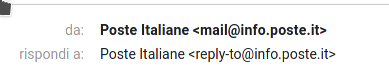
\includegraphics[width=.5\textwidth]{img/phishing/mittente}
    \item Messaggio inviato \textbf{tramite} un server diverso \\
      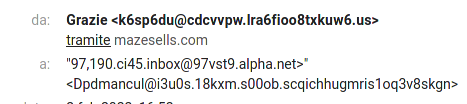
\includegraphics[width=.5\textwidth]{img/phishing/destinatario}
    \item L'indirizzo di risposta è diverso dal mittente
  \end{itemize}

  \medskip\only<+->{
  \textbf{Attenzione} il mittente di una mail si può falsificare!}
\end{myframe}

\begin{myframe}{Attenzione al destinatario}
  \begin{itemize}[<+->]
    \item Destinatario è newsletter \\
      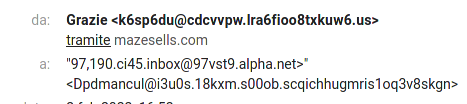
\includegraphics[width=.5\textwidth]{img/phishing/destinatario}
    \item Non c'è destinatario, ma Ccn (copia carbone nascosta) \\
      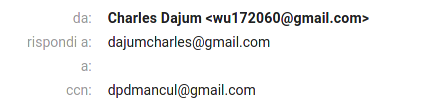
\includegraphics[width=.5\textwidth]{img/phishing/ccn}
  \end{itemize}
\end{myframe}

\begin{myframe}{Attenzione all'indirizzo del sito}
  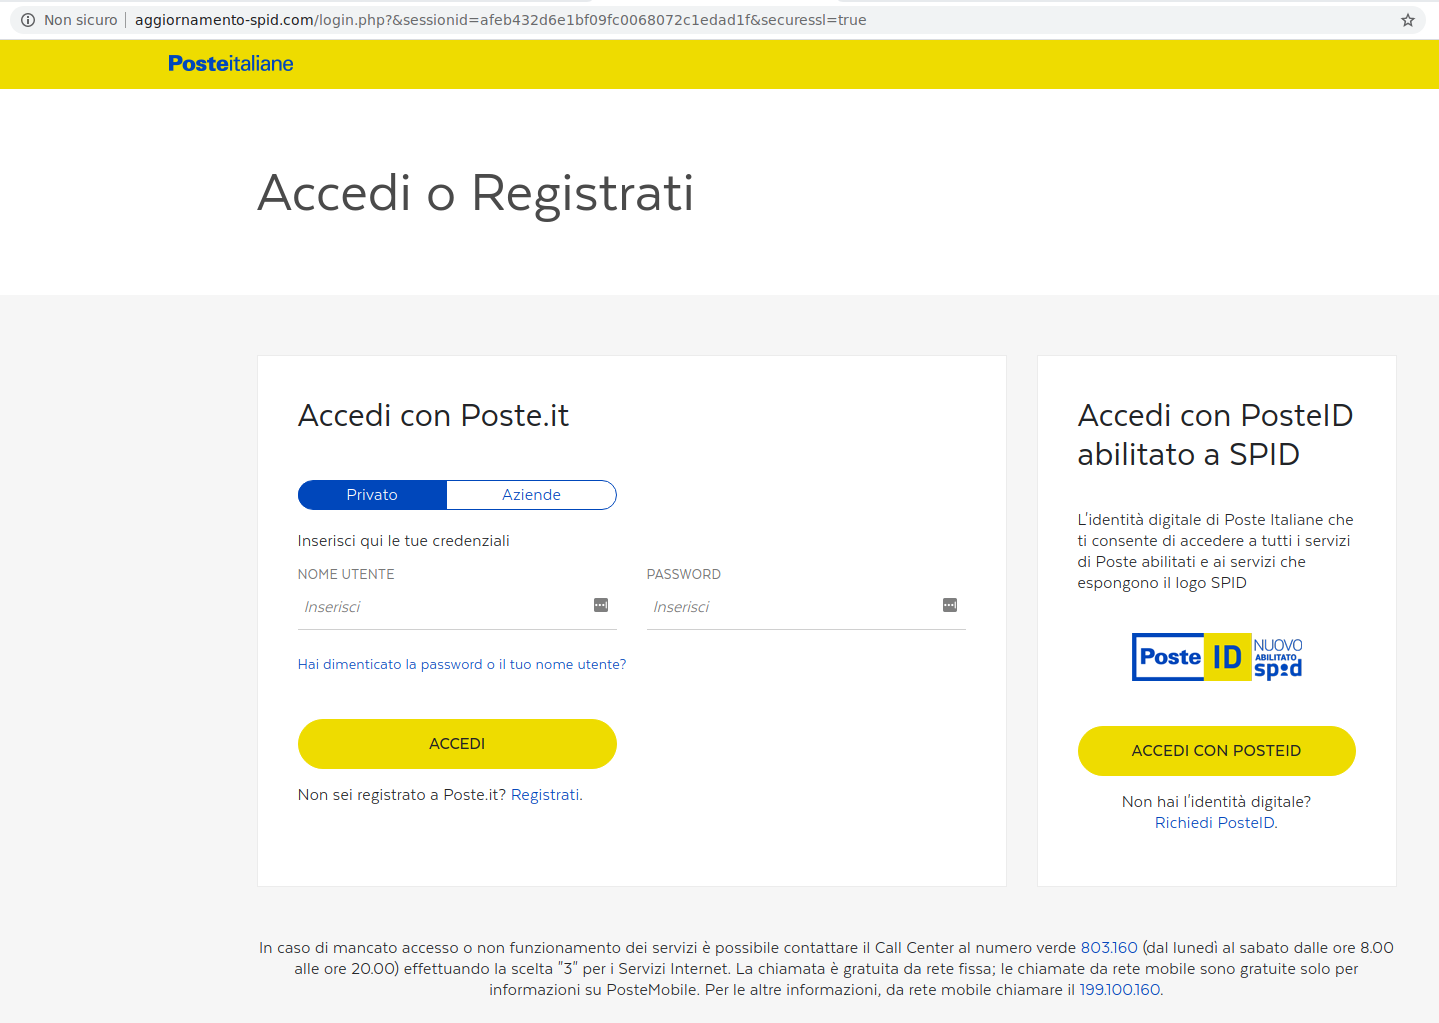
\includegraphics[width=.8\textwidth]{img/phishing/url}
\end{myframe}

\begin{myframe}{Il protocollo https}
  La \emph{s} in https sta per \textbf{sicuro}. Https è infatti la versione crittografata di http:\\nessuno può intercettare la comunicazione.

  \medskip\pause
  Se un sito usa il protocollo \textbf{http} (senza s) \textbf{non inserire mai password} e dati sensibili: chiunque sulla rete può leggerli!
\end{myframe}

\begin{myframe}{Pagamenti sicuri}
  Per evitare di \textbf{farsi rubare i dati delle carte}\\è sempre meglio usare \textbf{intermediari affidabili} nei pagamenti.

  \pause\bigskip
  Ad esempio PayPal offre anche una garanzia di rimborso in caso di truffa.
\end{myframe}

